\chapter{Conditional Sum}

Conditional sum is a divide and conquer algorithm, and hence exploits binary tree parallelism.  The algorithm works by calculating both possible results for each bit (if carry in was 1 or 0), then performing paired conditional concatenation using the actual carry bit of the lower number, see Figure~\ref{f-cond_sum_add}.

\begin{figure}
\caption{Conditional Sum Adder (above), and its sub-blocks (below, left and right).}\label{f-cond_sum_add}
\begin{center}
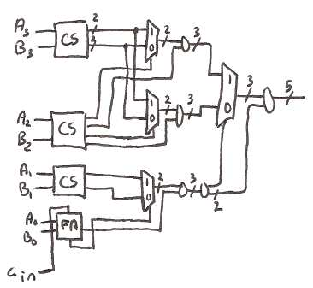
\includegraphics{conditional_sum.png}\\\vspace{.2in}
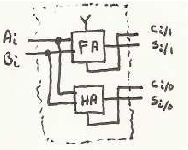
\includegraphics{cs_4out.png} \hspace{.2in} 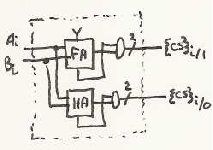
\includegraphics{cs_2out.png}
\end{center}
\end{figure}

\begin{enumerate}
    \item form conditional terms for each digit in summation $\rightarrow$ (digit with carry, digit without carry) = ($x_i+y_i+1$,$x_i+y_i$)
    \item group by twos from right and for both conditional values in the right parenthesis form the result as follows:
    \begin{enumerate}
        \item the leftmost bit of the two terms on the right are the carry bits used to select the term on the left
        \item concatenate the appropriate term on the left (picked by carry) with each term on right after removing the parity bits of the right terms
    \end{enumerate}
    \item continue pairings until only 1 term remains. pick right number if $c_{in}=0$ else pick left.
\end{enumerate}

\begin{example}
 Add $x=0110$ and $y=1111$ by conditional sum and indicate if overflow occurred.

        {\color{ans}
        \begin{tabular}{cccc}
          0+1 & 1+1 & 1+1 & 0+1 \\
          $\downarrow$ & $\downarrow$ & $\downarrow$ & $\downarrow$ \\
          (10,01) & (11,10) & (11,10) & (10,01) \\
          $\searrow$ & $\swarrow$ & $\searrow$ & $\swarrow$ \\
          \multicolumn{2}{r}{(101,100} & \multicolumn{2}{l}{(110,101)} \\
          \multicolumn{2}{c}{$\searrow$} & \multicolumn{2}{c}{$\swarrow$} \\
          \multicolumn{4}{c}{(10110,10101)} \\
          \multicolumn{4}{c}{1 0101} \\
        \end{tabular}

        No overflow occurred (added a positive and negative number).
        }
\end{example}



\begin{example}
    Calculate $7-8$ by conditional sum.

    {\color{ans}

    $7=0111$ and $-8=1000$

    \begin{tabular}{cccc}
    $\;$ 0       & 1          & 1          & 1          \\
      +1         & 0          & 0          & 0          \\ \hline
      (10,01)    & (10,01)    & (10,01)    & (10,01)    \\
      $\searrow$ & $\swarrow$ & $\searrow$ & $\swarrow$ \\
      \multicolumn{2}{c}{(100,011)} & \multicolumn{2}{c}{(100,011)} \\
      \multicolumn{2}{c}{$\quad\searrow$} & \multicolumn{2}{c}{$\swarrow\quad$} \\
      \multicolumn{4}{c}{(10000,01111)} \\
    \end{tabular}

    Since this was done as addition no carry-in was set so the solution is \begin{tabular}{r|l} 0 & 1111 \\ \hline \end{tabular} or $-1$ in signed base ten.

    }
\end{example}


\begin{example}
Add by conditional sum $x=01100110$ and $y=00110011$.

{\color{ans}
\noindent
\begin{tabular}{rrrrrrrr}
$0+0$ & $1+0$ & $1+1$ & $0+1$ & $0+0$ & $1+0$ & $1+1$ & $0+1$ \\
$\downarrow$ & $\downarrow$ & $\downarrow$ & $\downarrow$ & $\downarrow$ & $\downarrow$ & $\downarrow$ & $\downarrow$ \\
$(01,00)$ & $(10,01)$ & $(11,10)$ & $(10,01)$ & $(01,00)$ & $(10,01)$ & $(11,10)$ & $(10,01)$ \\
$\searrow$ & $\downarrow$ & $\searrow$ & $\downarrow$ & $\searrow$ & $\downarrow$ & $\searrow$ & $\downarrow$ \\
\multicolumn{2}{r}{$(010,001)$} & \multicolumn{2}{r}{$(110,101)$} & \multicolumn{2}{r}{$(010,001)$} & \multicolumn{2}{r}{$(110,101)$} \\
& $\searrow$ & & $\swarrow$ & & $\searrow$ & & $\swarrow$  \\
&  & \multicolumn{2}{c}{$(01010,01001)$} &  &  & \multicolumn{2}{c}{$(01010,01001)$ }  \\
&  &  & $\searrow$ &  & $\swarrow$ &  &  \\
&  &  & \multicolumn{3}{c}{$(010011010,010011001)$} &  &  \\
&  &  & \multicolumn{3}{c}{$0 \, 10011001$} &  &  \\
\end{tabular}
}
\end{example}

Why go through this?  First, by a folk theorem of Dr. Alan Laub, ``\emph{What is hard for us tends to be easy for computers (and vice versa)}.''  In reality this process is really easy for a computer to do.  Second, the process is highly parallel, so it can be done very fast.  If the numbers to be added are n bits long this takes $2(\log_2(n)+1)$ levels of logic, much better than the $n+1$ levels of logic required by ripple calculations.  Thus it is O(log(n)) in time complexity.  For example, for adding the 32 bit numbers considered already, conditional sum would take $2(\log_2(32)+1)=12$ levels of logic, so on the fast logic described it would be 12ns, a huge improvement.

